\chapter{Lavon Perrin: Mindset, Time Windows, and the Replication Test}

This chapter follows the School of Hard Knocks interview with Lavon Perrin, curated by LazyingArt LLC through Video2Book, as a source-conscious case study in commercial judgment. The source is not a blackboard lecture; no validated mathematical frames remain. The mathematical content is therefore modest and practical: a time-zone calculation, a goal-size comparison, a replication test for scale, and a final distinction between money as a number and money as managed freedom.

\section{The Opening Rule: Who You Stand Near}

The episode opens before the formal introduction. Perrin begins with a rule from his mother: if you hang around nine broke friends, you are going to be the tenth. If you hang around nine people driving Ferraris, he says, your odds are better.

That is not a theorem. It is an anecdotal law of surroundings. But it is also the governing motif of the interview. Perrin will return to the same structure when he talks about mindset, licensing, moving downtown, risk, reading, time, and money. The person is never treated as isolated from the inputs around him.

The simplest notation for the opening rule is deliberately elementary:

\begin{equation}
9+1=10.
\end{equation}

The arithmetic is not the proof of the claim; it is the shape of the claim. In Perrin's telling, the tenth person is not merely adjacent to the nine. The tenth person is being trained by them: by their standards, vocabulary, habits, and accepted limits.

\begin{remark}
The transcript appears to garble some later car references. The notes preserve the peer-environment mechanism without relying on exact counts of Ferraris or Porsches.
\end{remark}

Only after this cold open does James Doolin introduce the School of Hard Knocks series, ``10 Questions with Millionaires,'' and name Perrin as the first guest. The opening question is broad: what separates people in business from their peers?

\section{Mindset as the First Tool}

Perrin's answer is almost immediate: mindset. If he were building a person and could put only one major tool inside that person, he says, it would be mindset.

The answer matters because of what it excludes. He does not begin with capital, tax structure, sales scripts, or a product category. He begins with interpretation. A situation can be read as negative or workable. A person can feed the mind with constant negative information or deliberately keep some of it out. Perrin's own example is simple: he does not watch the news because he does not want to live inside that stream of negativity.

\subsection{Question \& Answer}

\paragraph{Question.}
If mindset is the answer, what does it actually change?

\paragraph{Answer.}
In this interview, mindset changes the first explanatory move. Perrin's test is the mirror. If we are not where we want to be, the first question is not only what the market did, what the boss did, or what the economy did. The first question is what we could have done differently.

A cautious note-writing shorthand is:

\begin{equation}
R_{t+1}
=
R_t
+
A\!\left(M_t,I_t\right),
\end{equation}

where \(R_t\) is the present result, \(M_t\) is the mindset or accountability state, \(I_t\) is the information environment, and \(A\) is the next action. This is not a behavioral law. It is a compact way to remember Perrin's sequence: information shapes interpretation; interpretation shapes accountability; accountability shapes action.

The interview then turns from mindset as an attitude to mindset as an operating move. Perrin says to go with a group, then gives the side-hustle example.

\section{Buying Time With Geography}

The clearest arithmetic in the interview is the East Coast--West Coast licensing example. Perrin says that some people living on the East Coast buy a license on the West Coast. That buys them three hours a day.

The ordinary day remains ordinary: work from 9 to 5, have dinner, take care of children or evening obligations. Then, around 8 p.m. local time, when the East Coast calling window is effectively closed, the West Coast is still open.

\begin{align}
T_{\mathrm{local\ stop}} &= 8{:}00\ \mathrm{p.m.},\\
\Delta_{\mathrm{zone}} &\approx 3\ \mathrm{hours},\\
T_{\mathrm{last\ call}} &= T_{\mathrm{local\ stop}}+\Delta_{\mathrm{zone}}
= 11{:}00\ \mathrm{p.m.}.
\end{align}

So the mechanism is not just ``work harder.'' It is more exact: change the reachable market so that the same evening contains more available selling time.

\begin{figure}
\centering
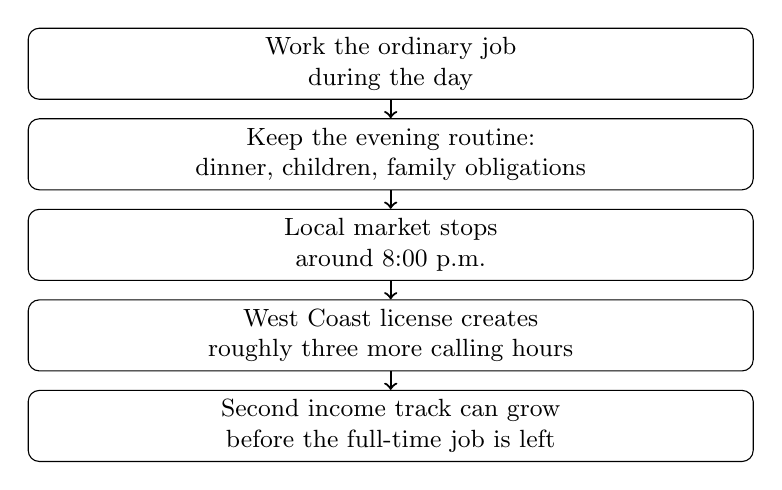
\begin{tikzpicture}[
  every node/.style={font=\small},
  box/.style={
    draw,
    rounded corners,
    align=center,
    text width=0.74\linewidth,
    minimum height=0.74cm
  },
  arrow/.style={->, thick}
]
\node[box] (job) at (0,0) {Work the ordinary job\\during the day};
\node[box] (family) at (0,-1.15) {Keep the evening routine:\\dinner, children, family obligations};
\node[box] (local) at (0,-2.30) {Local market stops\\around \(8{:}00\) p.m.};
\node[box] (west) at (0,-3.45) {West Coast license creates\\roughly three more calling hours};
\node[box] (career) at (0,-4.60) {Second income track can grow\\before the full-time job is left};
\draw[arrow] (job) -- (family);
\draw[arrow] (family) -- (local);
\draw[arrow] (local) -- (west);
\draw[arrow] (west) -- (career);
\end{tikzpicture}
\caption{The time-window mechanism: a later market turns an ordinary evening into a second selling period.}
\end{figure}

This is one of the most concrete claims in the interview. Opportunity is created not by a new motivational phrase, but by a different map of time.

\section{The Turn Toward Ownership}

The interviewer next asks for the turning point. Perrin does not answer with a single dramatic instant. He says it ``just kind of happened.'' Corporate America did not feel like a fit. He had questions, he pushed against the system, but he was good at sales, people liked him, and he could lead.

\subsection{Question \& Answer}

\paragraph{Question.}
Was there one decisive turning point?

\paragraph{Answer.}
No single moment is presented as the whole explanation. Perrin describes accumulation. He learned how businesses worked while employed by other companies. Then he wanted to take those tools and use them for himself. The car business added a personal constraint: he did not want the lifestyle he associated with that world, and he wanted to see his kids.

We can write the local transition as:

\begin{equation}
\mathrm{employment\ learning}
+
\mathrm{family\ constraint}
+
\mathrm{sales\ ability}
\longrightarrow
\mathrm{ownership\ attempt}.
\end{equation}

The arrow should be read as narrative mechanics, not destiny. Perrin is describing why ownership became the structure that fit the life he wanted to build.

\section{Scaling by Raising the Target and Testing the Operator}

The next question asks what enabled him to scale. Perrin begins with a number: many people want to make \(\$100{,}000\) a year. His response is that if the plan were built for \(\$500{,}000\), then even missing the target might still leave a person near \(\$100{,}000\).

\begin{equation}
G_{\mathrm{common}}=\$100{,}000,\qquad
G_{\mathrm{plan}}=\$500{,}000,\qquad
G_{\mathrm{plan}}=5G_{\mathrm{common}}.
\end{equation}

The point is not that a larger number magically produces a larger result. The point is that the number changes the design problem. A \(\$100{,}000\) wish may tolerate one operating system. A \(\$500{,}000\) plan asks for another.

\subsection{Question \& Answer}

\paragraph{Question.}
Why would a larger goal change the result?

\paragraph{Answer.}
Because the plan must be built to the goal. Perrin's claim is that a larger target forces questions about volume, skill, accountability, and repeatability. Missing a large plan may still land higher than succeeding at a small wish, but only because the larger plan changed behavior first.

His next test is the replication question: would the company, customer, or business partner be happy if there were ten of him?

\begin{equation}
N_{\mathrm{copies}}=10.
\end{equation}

This is the operator test. If one version of the operator is valuable, ten copies suggest scale. If ten copies would create confusion, unreliability, or weak service, then scale is premature. The unit has to be worth multiplying.

\begin{table}
\centering
\begin{tabular}{|p{0.40\linewidth}|p{0.46\linewidth}|}
\hline
\textbf{Transcript-backed test} & \textbf{Commercial meaning} \\
\hline
\(\$100{,}000\) desired income & A common target that may be paired with too small a plan. \\
\hline
\(\$500{,}000\) planned income & A larger design problem that can force different action. \\
\hline
``Ten of me'' & A replication test for reliability, value, and scale. \\
\hline
\end{tabular}
\caption{Perrin's scale logic: raise the design target, then test whether the operator is worth multiplying.}
\end{table}

At this point the opening rule returns. Perrin talks about putting himself around successful people, moving downtown, and being near people living the kind of life he wanted. The environment is not an inspirational backdrop. It is treated as part of the scaling apparatus.

\section{Risk, Sales, and Personal Development}

The interviewer then asks about risk. Perrin gives a blunt answer: there is no success without risk. But his risk is not blind exposure. It is calculated risk, paired with learning, self-belief, and education.

A compact reconstruction is:

\begin{equation}
\mathrm{useful\ risk}
=
\mathrm{calculation}
+
\mathrm{learning}
+
\mathrm{commitment}.
\end{equation}

The next question asks how someone in sales can succeed. Perrin does not offer a closing trick or a script. He says personal development. He did not read much in his youth or after college, though he took online classes in the early 2000s and earned his degree. Later, reading helped validate thoughts and ambitions he already had but did not yet understand.

The numerical detail should stay in the notes:

\begin{equation}
B_{\mathrm{last\ year}}\approx 15\ \mathrm{books}.
\end{equation}

He names \textit{Think and Grow Rich} by Napoleon Hill as the book that stands above the others for him. He also names \textit{Rich Dad Poor Dad} and \textit{Go for No}. The list is not generic decoration; it is evidence for how Perrin describes his own self-education. His mentor rereads \textit{Think and Grow Rich} every September, and Perrin frames his own rereading as part of that rhythm.

\begin{remark}
The reading claims should remain attached to Perrin's account. They are not proof that a particular book causes wealth; they are evidence that personal development became part of his operating discipline.
\end{remark}

\section{Mistakes, Time, and What Money Is For}

The later interview gathers the constraints that come after the initial push: consistency, budgeting, mistakes, time, and the meaning of money. Perrin says one of the hardest parts of owning a business is learning how to be a business owner. That means accepting ups and downs, learning where money should go, and not becoming frozen by overanalysis. He names the familiar trap: paralysis by analysis.

When asked about the worst financial decision he ever made, he resists the premise. He says decisions that do not go your way are not purely negative. They are like sports: you do not necessarily lose; you learn. Then he gives the BMW 750 story. He had wanted one since growing up mainly in Germany. He had the opportunity to own two. A mechanic in Austin warned him that buying one would make them good friends, because Perrin would be seeing him often. Perrin's conclusion is not total regret; it is that he should have bought differently, with a maintenance plan and better preparation.

The work-life balance question then turns into a time question. Perrin compares ordinary complaints about not having time with the output of people who run much larger enterprises. His point is not that everyone has the same responsibilities. It is that leverage changes what can be done with the same twenty-four hours: better use of time, better people around the work, better delegation.

\subsection{Question \& Answer}

\paragraph{Question.}
Does money buy happiness?

\paragraph{Answer.}
Perrin narrows the question. Money can buy freedom, he says, if a person knows what to do with it. But the amount alone is not the answer. If someone cannot manage \(\$1{,}000\), he says, that person cannot manage \(\$1{,}000{,}000\).

\begin{equation}
\$1{,}000{,}000 = 1000 \times \$1{,}000.
\end{equation}

This is the final management test. A larger number magnifies the same habits. Money becomes freedom only when the person can handle money.

\begin{figure}
\centering
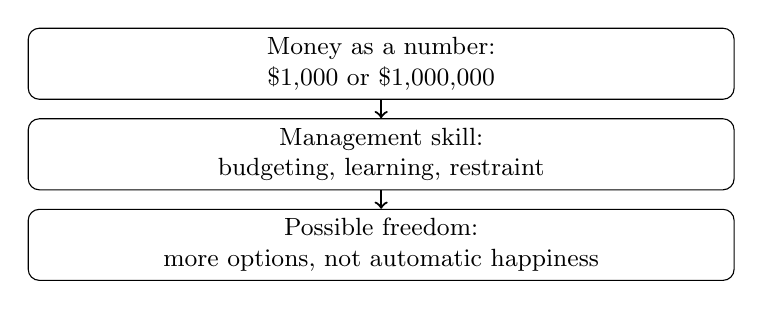
\begin{tikzpicture}[
  every node/.style={font=\small},
  box/.style={
    draw,
    rounded corners,
    align=center,
    text width=0.72\linewidth,
    minimum height=0.74cm
  },
  arrow/.style={->, thick}
]
\node[box] (money) at (0,0) {Money as a number:\\\(\$1{,}000\) or \(\$1{,}000{,}000\)};
\node[box] (skill) at (0,-1.15) {Management skill:\\budgeting, learning, restraint};
\node[box] (freedom) at (0,-2.30) {Possible freedom:\\more options, not automatic happiness};
\draw[arrow] (money) -- (skill);
\draw[arrow] (skill) -- (freedom);
\end{tikzpicture}
\caption{Perrin's final distinction: money can buy freedom only when money is managed.}
\end{figure}

\section{Summary}

The interview begins with surroundings and ends with management. Perrin's argument unfolds through practical tests rather than abstract doctrine: choose the inputs around the mind, buy time through geography, leave a structure that no longer fits, scale only what is worth copying, take calculated risk, learn deliberately, and treat money as freedom only when it is managed.

The mathematics is bookkeeping mathematics, but it keeps the mechanisms honest:
\[
8{:}00+3\ \mathrm{hours}=11{:}00,\qquad
\$500{,}000=5\times\$100{,}000,\qquad
N_{\mathrm{copies}}=10,
\]
\[
B_{\mathrm{last\ year}}\approx15,\qquad
\$1{,}000{,}000=1000\times\$1{,}000.
\]
None of these expressions proves wealth. They do something more local and more useful for these notes: they preserve the concrete claims in the interview and keep each slogan tied to an operating mechanism.